%\documentclass[11pt]{article}
%\usepackage[pdftex]{graphicx}
%\usepackage{rotating}
%\begin{document}

%\title{NuSIM and NuSTAR science. Quick Start Guide.}
%\author{Andreas Zoglauer and Kristin Kruse Madsen}
\chapter{NuSIM and NuSTAR science. Quick Start Guide.}
%\maketitle
One of the main goals of NuSIM is to predict, reproduce, and help understand NuSTAR measurements.
For these tasks NuSTAR can be considered as a black box, and the user only has to think about the required input data and the output data he gets from NuSIM. 

This chapter will give an overview of NuSIM's science capabilities, the required user inputs, how to perform the simulations, and the output the user can expect from NuSIM. This chapter therefore can be considered as a quick start guide to NuSIM.

\section{What NuSIM can do (and what not)}

NuSIM's strongest point is its imaging simulation capability. The NuSTAR observatory is very dynamical and a steady nominal observation is far from actually steady. The mast will go through an orbital bending cycle due to the sun/shade patterns on the mast, and this can in the worst case cause the effective area to change  by as much as 10\%. In addition there are other thermal perturbations which may affect the reconstruction of the source, increasing the PSF. All of these effects are included in NuSIM, and NuSIM will mimic a typical observation environment, then perform the typical aspect reconstruction on the data. The output will be an aspect reconstructed event list in sky coordinates, equivalent to a level 2 fits file.

NuSIM is very well suited to investigate tiling and pointing patterns of sources as it offers full control of how to orient and where to point the observatory. Also due to the detector gaps care should be taken to think about exact locations.

NuSIM will also correctly process the input spectrum of the source, running it through a detector engine that simulates the NuSTAR detector response. However, if the goal of the simulation is just to get the spectrum, then it is better to use XSPEC, since the choices in input spectrum are limited and a simulation may take several hours. NuSIM is not well suited to iterative investigations. It is therefore advised that investigations on what spectrum and integration time to use in a simulation, should be done prior to the simulation in XSPEC or a similar tool.


\begin{center}
\begin{tabular}{|p{9cm}|}
\hline
\hline \textbf{NuSIM is suitable for} : \\ 
\hline  
\hline
Pointing and tiling pattern simulations for extended fields. \\
\hline
Extended objects. \\
\hline
Pointing environmental stability. \\
\hline
Sensitivity studies.\\
\hline
\hline \textbf{NuSIM is not suitable for}: \\
\hline
\hline
Variability. NuSim can not simulate variable spectra. \\
\hline
Detailed spectral analysis. Very time consuming as any change in parameter requires a new simulation.\\
\hline
\end{tabular} 
\end{center}

\subsection{What NuSIM cannot do}
Currently NuSIM outputs an event list that can be loaded into DS9. Extractions can be made using FTOOLS, however, at the time NuSIM does not provide an ARF generation routine, so it is not possible to extract fluxes. At the time of writing we are trying to remedy that, but it is a complicated process that may not be imminently available.

NuSIM currently can not simulate variable sources, i.e. there is no way to input a time varying spectrum. Optionally though if a source is known to be in several different states at a certain fraction of time, then NuSIM can simulate each state separately, and the simulations can be stitched together afterwards.

Similarly NuSIM can not assign several different spectral shapes to an input image. Each input image can only have one spectrum assigned to it. If several spectrum exists then it becomes necessary to make an image for each spectrum and simulate them as separate source.

In any instance where one observation is composed of several individual simulations that must be added together in parallel (as opposed to stitching together simulations back to back), there will be an error in the absolute countrate. The reason is that the deadtime calculation depends on the total flux, but each sub simulation will have ran at a fraction of the total flux. For example an image of a source consisting of a core and a halo, that each has a different spectrum, should be broken up into two sub images. If each of the images is responsible for 50\% of the combined flux, the two simulations will be run with 50\% of the flux. The resulting countrate of each sub-simulation will be higher than the actual countrate had there been only one simulation with 100\% flux. The error in the countrate depends on the flux level, and will be significant for fluxes above 10 milicrabs. Below that it is negligible.  


\section{User science input}

NuSIM contains many more possible input options than are required for science simulations. 
Indeed, there are many possibilities to set wrong parameters.
In order to prevent this, NuSIM has an astrophysics mode, which will allow the user to only modify modules relevant for science simulations.
All other modules are set to standard values by loading them from a default astrophysics configuration file.
This has the advantage that the user still can use his or her old configuration files even if the default configuration a simulation module has changed.
In order to activate astrophysics mode, one has to start NuSIM using the "-p"-option: \emph{nusim -p $<$name of configuration file$>$}. 

\begin{figure}[bt]
  \begin{minipage}[c]{0.48\linewidth}
    \begin{center}
      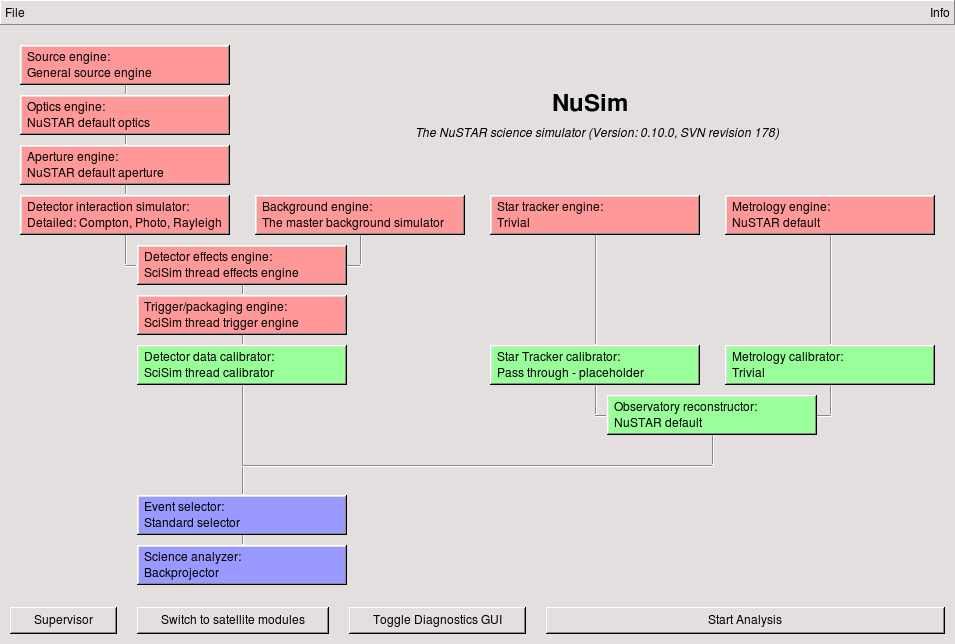
\includegraphics[scale=0.27]{images/MainWindowNormalMode.png}  
    \end{center}
  \end{minipage}
  \hspace{0.04\linewidth}
  \begin{minipage}[c]{0.48\linewidth}
    \begin{center}
      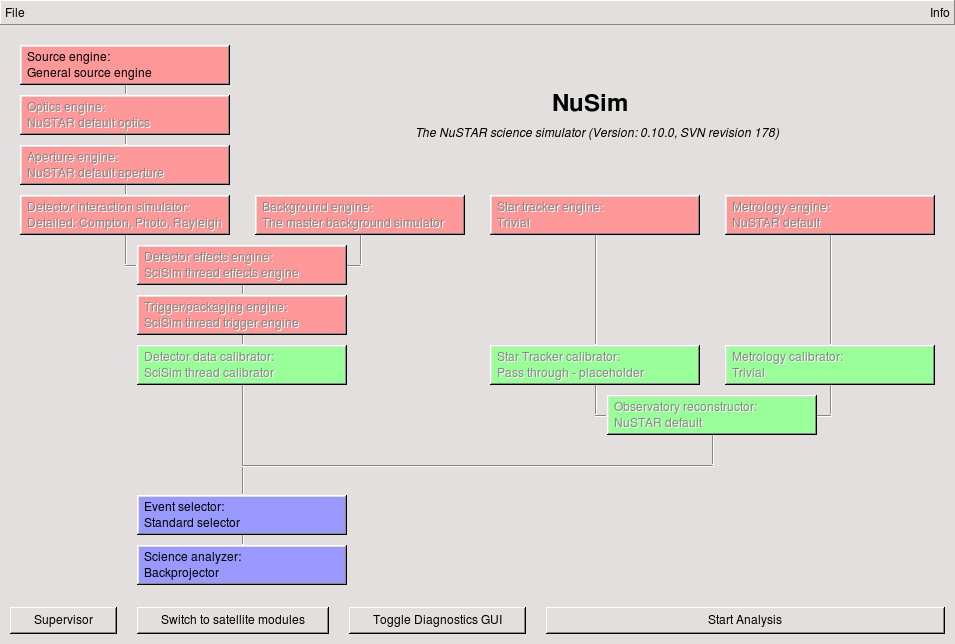
\includegraphics[scale=0.27]{images/MainWindowAstrophysicsMode.png}  
    \end{center}
  \end{minipage}
  \caption{\label{fig:mainwindowmodes} Illustration of the main NuSIM GUI window is normal (left) and astrophysics (right) mode: In the latter, only the source, event selection, and backprojection module are active. }
\end{figure}


Then only the following modules can be modified:
\begin{itemize}
\item The source module: 
It contains a list of sources which are defined by a name, a beam (e.g. far field point source, or a fits file) determining the origin directions, a spectrum, as well as a flux.
The beams relevant for science simulations are the far-field point source, which require the RA and DEC of the source, and the fits-image. The later is usually an image which has been measured by e.g. Chandra.
The spectrum is defined by its type, for example power law. 
After the type is selected, the user can set the other spectral options.
In the case of a power law this encompasses the minimum and maximum energy as well as the photon index.
The final parameter is the flux.
In order to enable simulations of various beam and spectral parameters, it is necessary to give the energy-integrated flux of each source in ph/s/cm$^2$. 
The user has to take care of the integration.
An exception is the special spectral option "Normalized function in ph/cm2/s/keV". 
There you give the spectrum in mathematical form, which must contain the correct normalization in a C/C++ compatible form such as "7.0e-6*pow(x/10, -1)*exp(-sqrt(x/2.2))".
Pay attention to use of "x" for energy and "e" not "E" for the exponent.
To set many sources at once, it is also possible to read them from an ASCII file using the "Import from file" button. 
The file is a space-delimited csv file with different columns. If you only have point sources with simple power laws, the columns are: source name (no white spaced allowed), beam type (1 = far-field point source), RA (deg), DEC (deg), spectral type (3 = power law), minimum energy (keV), maximum energy (keV), photon index, flux (ph/s/cm$^2$).
An example can be found in the resource/configurations directory: GalacticCenter.ImportExample.txt
\item The pointing module: 
It is located in the "satellite options" pane. 
Here you give the RA and DEC of the direction where NuSTAR should point. 
This should obviously be the direction of your sources.
If you do not click the "All times are absolute" button then you will be able to set the total observation time in the Supervisor and the times given in the pointing will be scaled.
Otherwise all times are absolute. 
If you have a more complex pointing situation, you can import a list of pointings from file.
One easy possibility is to generate a default pointing pattern file by clicking the "Pointing" button in the source module. 
This will generate a text file with different pointings which will cover the area of the sources given in the source generator. The file format is described in \ref{inputformats:pointing}.
\item The event selector:
The event selector has two tasks, to store the simulated events to file and to perform event cuts.
Currently only energy cuts are implemented.
The events can be stored in three formats, a fits file containing an event list which can be used with the standard fits tools, a ROOT file, or an ASCII file.
The user can also choose to store the events before or after the event cuts.
\item The supervisor:
In the supervisor you give the total observation time. 
If you have set absolute times in the pointing module, the simulation will be stopped if the last pointing is finished, or earlier if the observation time is over. 
\end{itemize}
The options of all others modules should be left at the standard settings --- unless you are really sure what you are doing.


\section{Performing simulations}

Performing simulations is as simple as pressing the "Start Analysis" button. 
As soon as all modules have initialized the diagnostics window will come up. 
Every module can have a diagnostics tab attached. 
The default ones are associated with the source module, the detector effects engine, and the backprojector.
Switching to the backprojector (the "Results" tab) will show backprojections of the simulated events as well as the simulated spectrum.
The GUI is updated after as many events as given in the supervisor GUI.
If this number is too low, the GUI is updated too frequently which will slow down the simulations.
The simulation can be stopped at any time by pressing the "Stop Analysis" button.
If a file is selected in the event selector then all events are not only displayed in the GUI, but in parallel also written to the file.
After the simulations is finished some useful summary information is printed to the screen.

\section{NuSIM science output}

NuSIM outputs the results of the simulation in a simple FITS OGIP compatible event list format, that has coordinates of the event in the standard FITS OGIP sky coordinates (X, Y), and pulse height PI in keV. In addition there is a GRADE keyword which currently specifies whether an event was:
\begin{itemize}
\item[1] A properly double bounced source photon
\item[2] A background photon
\item[3] A single bounce source photon (ghost ray)
\end{itemize} 

This allows the user to sort the list and make different energy and grade cuts. It should be stressed, however, that all three grades are part of the actual image.

The output file will not run cleanly in XSELECT due to the fact that XSELECT does not have a NuSTAR mission parameter file. To use XSELECT with the files it is necessary to download a mission parameter file not part of the general HEASOFT distribution. This file with directions can be found on the projectspaces site for NuSIM in the Simulations/Tools folder.

\section{Example simuations}
Shown here are two example simulations describing the input used to run them.

\subsection{Simulation of extended object}
When simulating an extended source the objective is usually looking for features such as filaments in a supernova remnant. If the source has already been observed with CHANDRA or XMM then the input to NuSIM may conveniently be a fits image from those observatories. If not then the object must be simulated with some external tool to create an intensity map of the source.

Once the choice of input image has been chosen, a spectrum for the source must be specified. The spectrum may be either of the NuSIM internal spectra, or input as a file. When the shape of the spectrum has been specified, a desired energy range must be chosen and the total flux calculated over that particular energy range. For example if a power-law with normalization 10 and photon index 2.1 is chosen over the energy range of 5-80 keV, the total flux is 1.47 ph/cm$^2$/sec. This number must be supplied with the spectrum parameters since inside NuSIM, normalization is not an input parameter of the models, but is instead contained in the total flux. In a similar way an input spectral file need not be in absolute units, but should be supplied with the total flux of the energy range over which the file is specified.

Only one spectrum can be assigned per image. If a source exhibits several different spectra the image must be decomposed into separate images, and each image assigned to a spectrum.

Finally due to the geometry of the detectors a pointing plan must be considered. Things to think about are the number of pointing's needed to cover the source, and placement with respect to detector gaps.

\subsection{Simulation of survey}
For the simulation of a survey typically the objects are considered point sources. In this instance a catalogue with locations of each source can be used. If in addition the source spectra can be approximated by the NuSIM supplied models, the model parameters can be loaded as list together with the source location. If the sources require a more complex spectra it is necessary to load the spectra for each source as a separate file.

When the shape of the spectrum has been specified, a desired energy range must be chosen and the total flux calculated over that particular energy range. For example if a power-law with normalization 10 and photon index 2.1 is chosen over the energy range of 5-80 keV, the total flux is 1.47 ph/cm$^2$/sec. This number must be supplied with the spectrum parameters since inside NuSIM, normalization is not an input parameter of the models, but is instead contained in the total flux. In a similar way an input spectral file need not be in absolute units, but should be supplied with the total flux of the energy range over which the file is specified.

For surveys pointing strategies are of great importance. Things to consider when designing a pointing strategy is how much each consecutive pointing should overlap, what rotation of the observatory, the integration time, etc. There are tools in NuSIM to help facilitate the optimal pointing when given the total size of the field to be surveyed, the total exposure time, and the amount of overlap.

%\end{document}
